\documentclass{beamer}
\usetheme{metropolis}

\usetheme{metropolis}
\usepackage{listings}

\lstdefinestyle{Python}
{
    language=Python,
    basicstyle=\ttfamily\scriptsize,
    keywordstyle=\color{blue}\ttfamily,
	otherkeywords={self,False},
    commentstyle=\color{green!60!black}\ttfamily,
    stringstyle=\color{red!80!black}\ttfamily,
    backgroundcolor=\color{blue!10!white},
    showstringspaces=false,
    numbers=none,
    numberstyle=\tiny,
    numbersep=5pt,
    xleftmargin=2pt,
    framexleftmargin=4pt,
    framexrightmargin=4pt,
    framexbottommargin=5pt,
    framextopmargin=5pt,
    %breaklines=true,
    captionpos=b
}

\lstdefinestyle{MATLAB}{
    language=MATLAB,
    basicstyle=\ttfamily\scriptsize,
    keywordstyle=\color{blue}\ttfamily,
	otherkeywords={classdef,properties,methods},
    stringstyle=\color{red!80!black}\ttfamily,
    commentstyle=\color{green!60!black}\ttfamily,
    numbers=none,
    backgroundcolor=\color{orange!15!white},
    showstringspaces=false,
    numbers=none,
    numberstyle=\tiny,
    numbersep=5pt,
    xleftmargin=2pt,
    framexleftmargin=4pt,
    framexrightmargin=4pt,
    framexbottommargin=5pt,
    framextopmargin=5pt,
    %breaklines=true,
    captionpos=b
}

\lstdefinestyle{output}{
    language=bash,
    basicstyle=\ttfamily\scriptsize,
    keywordstyle=\ttfamily,
    stringstyle=\ttfamily,
    commentstyle=\color{green!60!black}\ttfamily,
    numbers=none,
    backgroundcolor=\color{white},
    showstringspaces=false,
    numbers=none,
    numberstyle=\tiny,
    numbersep=5pt,
    xleftmargin=2pt,
    framexleftmargin=4pt,
    framexrightmargin=4pt,
    framexbottommargin=5pt,
    framextopmargin=5pt,
    %breaklines=true,
    captionpos=b
}

\renewcommand{\emph}[1]{{\color{red}#1}}

\beamerdefaultoverlayspecification{<+->}

\setbeamercolor{block body}{bg=mDarkTeal!30}
\setbeamercolor{block title}{bg=mDarkTeal,fg=black!2}

\title{Test-Driven Development}
\author{Joachim Vandekerckhove}
\date{}


\newcommand{\module}[1]{{\color{brown}\texttt{#1}}}
\newcommand{\code}[1]{{\color{blue}\texttt{#1}}}
\newcommand{\name}[1]{{\color{violet}{#1}}}

\author{Joachim Vandekerckhove}
\date{}

\usepackage{graphicx}
\begin{document}

\title{Numerical integration}
\begin{frame}
  \maketitle
\end{frame}

\begin{frame}{Motivating application}
In cognitive science (and science generally), we are often interested in \emph{the probability that a theory is true} or the \emph{probability of values of parameters}.\\[2ex]

``Now that we have these data, what are the likely values of the generating parameters?''
\end{frame}


\begin{frame}[fragile]{Motivating application: Signal detection}
What is the probability distribution of $a$, assuming that
$$
\forall i: 
\left\{
\begin{array}{rcl}
\theta^f_i & = & \frac{f_i}{N}\\
\theta^h_i & = & \Phi\left(a + \Phi^{-1}\!\left(\theta^f_i\right)\right)\\
f_i &\sim& \text{Bin}\left(\theta^f_i, N\right)\\
h_i &\sim& \text{Bin}\left(\theta^h_i, S\right)\\
\end{array}
\right.
$$
and given the data $D$, which consists of hits $h_i$, false alarms $f_i$, signal count $S$, and noise count $N$?\\[2ex]
In other words, what is $p\left(a | D\right)$?
\end{frame}

\begin{frame}{Motivating application: Signal detection}
We can actually work out that distribution:
$$
p\left(a | D\right) = \frac{p\left(D|a\right)p\left(a\right)}{p\left(D\right)} \propto p\left(D|a\right)p\left(a\right)
$$
But now what?  We may want to \emph{characterize this distribution}:
\begin{itemize}
\item Get the mean of this distribution as a good guess for $a$
\item Calculate the probability that it is in a certain range
\item Get its standard deviation for a measure of uncertainty
\end{itemize}
\end{frame}


\begin{frame}{Motivating application: Signal detection}
\begin{itemize}
\item Get the mean of this distribution as a good guess for $a$: $$E(a | D) = \int_{-\infty}^{+\infty} a\, p(a | D)\;da$$
\item Calculate the probability that it is in a certain range: $$P(L < a < U | D) = \int_L^U p(a | D)\;da$$
\item Get its standard deviation for a measure of uncertainty: $$S(a | D) = \sqrt{E(a^2) - \left[E(a)\right]^2}$$
\end{itemize}
\end{frame}



\section{Numerical integration methods}


\begin{frame}{Some basic methods}
\begin{itemize}
\item The \emph{trapezoid rule}
\begin{itemize}
\item Divide the domain into small intervals
\item Approximate the curve over each interval by a simple shape
\item Approximate the integral by adding areas of the simple shapes
\end{itemize}
\item \emph{Gaussian quadrature}
\begin{itemize}
\item Only for curves of the form $f(x)\phi(x)$
\item Evaluate the curve at well-chosen quadrature points
\item Approximate the integral with a weighted average
\end{itemize}
\item \emph{Monte Carlo methods}
\begin{itemize}
\item Draw random samples that fall under the curve
\item Characterize the curve with summary statistics of the sample
\end{itemize}
\end{itemize}
\end{frame}



\section{Monte Carlo methods}

\frame{\frametitle{Numerical integration}
A very convenient approximation to the expectation integral is
\begin{eqnarray*}
   E(a | D) &=& \int_{-\infty}^{+\infty}a \, p(a | D)\;da\\
       &\approx& \frac{1}{R}\sum_{r=1}^{R}a_r \mbox{ where } 
                        \forall r: a_r \stackrel{iid}{\sim} p(a | D)
\end{eqnarray*}\pause
That is, the sample mean of a (large) random sample drawn from the distribution. 
Other summary statistics (like standard deviation) can be computed in a similar way.
This property is known as \emph{ergodicity}.\\[2ex]
\pause
It follows that in order to characterize an arbitrary distribution, it suffices
to be able to draw random samples from it.
}




\frame{\frametitle{Monte Carlo methods}
\begin{itemize}
 \item Sampling-based methods for describing distributions are called 
\emph{Monte Carlo methods} and they are extremely useful.
 \item They are called Monte Carlo methods after the famous casino in Monaco where a relative of the method's creator, \name{Stanislaw Ulam}, enjoyed gambling.
 \item Their initial development in 1947 almost immediately followed the completion of \name{ENIAC}, the first general-purpose digital computer, in 1945.
 \item There are many MC methods, but the most common ones are \emph{Markov chain Monte Carlo} (MCMC) methods.
\end{itemize}
}


\let\instr\texttt

\frame{\frametitle{Metropolis sampler}
\begin{itemize}
 \item A widely applicable algorithm is the \emph{Metropolis} algorithm.
 \item Named after \name{Nicholas Metropolis}, who created it together with \name{John von Neumann} while working on the \name{Manhattan Project}.
 \item In the algorithm, we will randomly generate \emph{candidate samples} from some simple distribution, and then decide to accept or reject the candidate.
 \item Metropolis algorithms need some customization and fine-tuning to be most efficient.
\end{itemize}
}

\frame{\frametitle{Metropolis sampler: Pseudocode}
Given a \emph{target} function $f(\theta) \propto p(\theta|D)$ and a symmetric
\emph{candidate generating distribution} $Q(x|y)=Q(y|x)$, a
Metropolis sampling algorithm proceeds as follows:
\begin{itemize}
 \item[1] \instr{Set} $i \leftarrow 1$ and \instr{choose} \emph{sample size} $R$
 \item[2] \instr{Choose}, arbitrarily, \emph{initial state} $\theta^{(0)}$
 \item[3] \instr{Draw} a randomly selected \emph{proposal} $\theta^{c}$ from $Q\left(\theta|\theta^{(i-1)}\right)$
 \item[4] \instr{Compute} the acceptance ratio $\alpha = \frac{f\left(\theta^{c}\right)}{f\left(\theta^{(i-1)}\right)}
 = \frac{p\left(\theta^{c}|D\right)}{p\left(\theta^{(i-1)}|D\right)}$
 \item[5] \instr{Draw} a randomly selected \emph{uniform variate} $u$ from $U(0,1)$. \instr{If} $\alpha > u$, 
          \instr{set} \emph{state} $\theta^{(i)} \leftarrow \theta^{c}$, 
          \instr{otherwise set} \emph{state} $\theta^{(i)} \leftarrow \theta^{(i-1)}$
 \item[6] \instr{Set} $i \leftarrow i + 1$. \instr{If} $i \leq R$, \instr{return} to Step~3, 
          \instr{otherwise halt}
\end{itemize}
}

\frame{\frametitle{Metropolis sampler: Common choices}
\begin{itemize}
 \item $R$ will often be large, like 5,000.
 \item $Q()$ will often be something that's easy to sample, like a normal distribution.
 \item $p(\theta|D)$ will often be our posterior distribution.
 \item Often, for computational stability, we will deal with $\log\left(p(\theta|D)\right)$, in which case we come the log of the acceptance probability $\log(\alpha) = \log\left(p(\theta^c|D)\right) - \log\left(p(\theta^{(i-1)}|D)\right)$ and compare it to the log of a uniform variate, $\log(u)$.
\end{itemize}
}

\frame{\frametitle{Metropolis sampler: Adaptation}
\begin{itemize}
  \item Using a normal distribution as the candidate generating distribution brings an advantage:  we can choose the width of it so that the CGD envelops the target distribution tightly.
  \item That way, more samples can be accepted and the algorithm can be more efficient.
  \item We will \emph{tune} the sampler so that it accepts approximately 40\% of all proposed samples.
  \item During the \emph{adaptation phase}, we will ``warm up'' the algorithm but the samples drawn during this phase are not yet samples from the target distribution, so we discard them.
\end{itemize}
}

\frame{\frametitle{Metropolis sampler: Adaptation}
\begin{itemize}
  \item The \emph{adaptation phase} goes like this:
\begin{enumerate}
  \item Run the sampler for some iterations $n_k$ and keep track of the \emph{acceptance rate $r_k$}: the fraction of samples that gets accepted
  \item If that fraction is too low, decrease the standard deviation because it's jumping around too wildly
  \item If it is too high, increase the standard deviation because it's climbing a slope  
  \item Repeat this a few times to get an acceptance rate close to 40\%
\end{enumerate}
\item A simple rule to update the standard deviation is $$\sigma_\text{new} = \sigma_\text{old} \times \left(\frac{r_\text{target}}{r_k}\right)^{1.1}$$
\item How much to fine-tune depends on the specific case.
\end{itemize}
}


\frame{\frametitle{Metropolis sampler: Post-processing}
\begin{itemize}
 \item We have to make sure the chain has converged to a stationary sampling state before using the samples for inference.
 \item Often, we will discard a number of initial samples known as the \emph{burn-in}:
 $$\hat a = \frac{1}{R-B} \sum_{i=B+1}^R a^{(i)}$$
\end{itemize}\null\vspace{0pt}
\centering
\scriptsize \bfseries{Trace plot}
\framebox{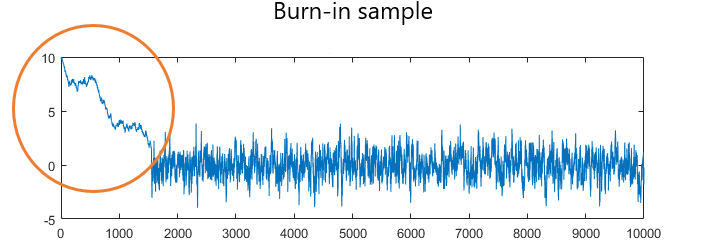
\includegraphics[width=.9\textwidth,trim=0 0 0 25pt,clip]{figures/burn-in.png}}
}


\frame{\frametitle{Metropolis sampler: Diagnostics}
\begin{itemize}
 \item We usually also repeat the procedure a few times with different values for $\theta^{(0)}$ to ensure that the algorithm converges to the same stationary distribution.
 \item Several convergence statistics exist, with \name{Geweke's} and \name{Gelman's $\hat R$} being the most popular.
\end{itemize}
\centering
\scriptsize \bfseries{Trace plot}\\
\framebox{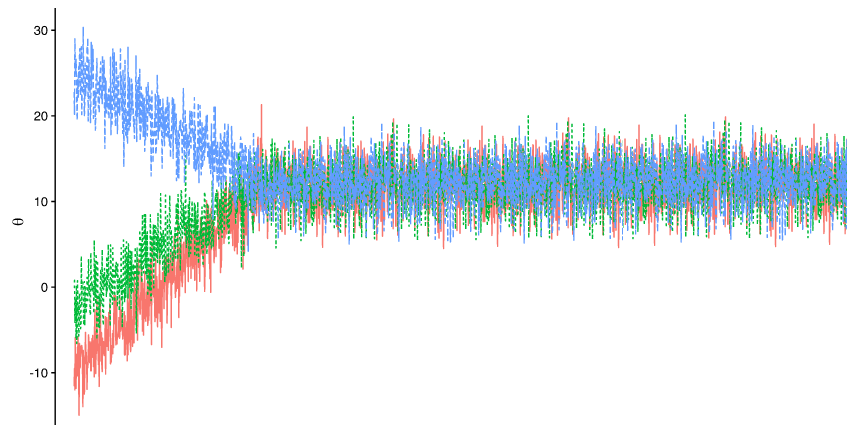
\includegraphics[width=.75\textwidth,trim=70pt 0 0 25pt,clip]{figures/convergence.png}}
}


\frame{\frametitle{Metropolis sampler: Inference}
\begin{itemize}
 \item Finally, we calculate the quantities we're interested in using.
 \item The quantities can be simple summaries of the samples in our MCMC chain (mean, median, standard deviation, probabilities in intervals, quantiles...).
 \item However, they can also be complex functions of the samples, such as \emph{posterior predictives} -- entire simulated data sets:
 \begin{enumerate}
  \item Draw samples
  \item Generate a synthetic data set from each sample
  \item Calculate a summary statistic on each synthetic data set and visualize the distribution
  \item Calculate the same statistic on the real data and show its position in the distribution
 \end{enumerate}
 \item Figures can also be summary statistics!
 \begin{enumerate}
   \item[--] You could draw a curve to visualize your data and then draw a distribution of synthetic curves using your sampled parameters
   \end{enumerate}
\end{itemize}
}


\frame{\frametitle{Metropolis sampler: Inference}
\setlength{\unitlength}{1pt}
{
\begin{picture}(300,200)
\put(-15,80){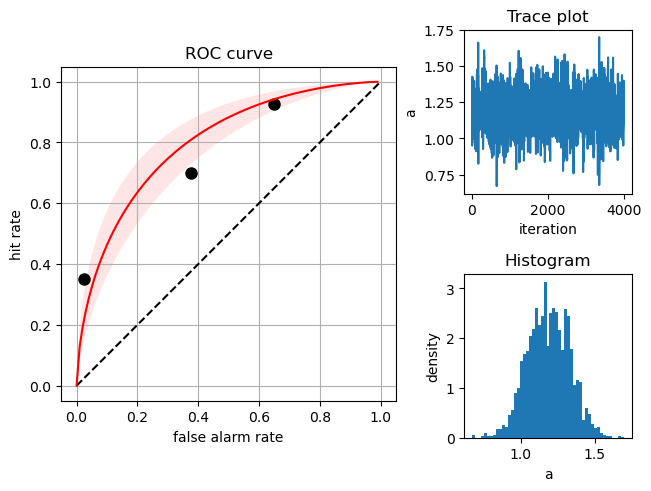
\includegraphics[width=.5\textwidth]{/home/joachim/Dropbox/Teaching/cogs106/7-integration/assignment/rocResults.png}}\pause
\put(150,0){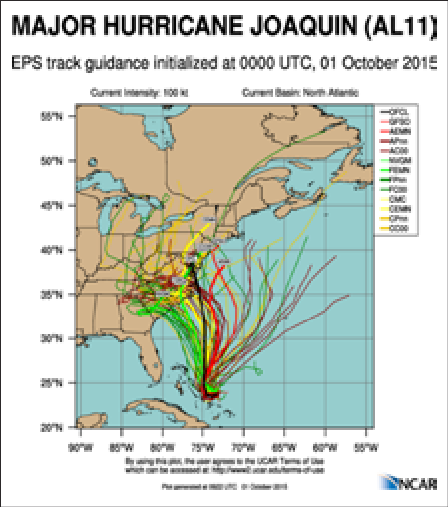
\includegraphics[width=.55\textwidth,trim=0pt 0 0pt 0pt]{figures/hurricane-joaquin.png}}\pause
\put(-10,-20){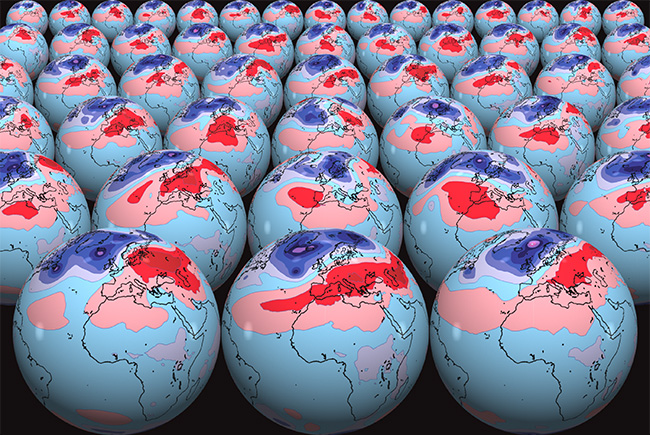
\includegraphics[width=.45\textwidth,trim=0 0 0 0]{figures/many-worlds-climate.jpg}}
\end{picture}
}
}

\frame{\frametitle{Metropolis sampler: Overview}
Typical steps of a Metropolis analysis are thus:
\begin{enumerate}
 \item \emph{Set up:} Select target function $f(\theta)$ and initial state $\theta^{(0)}$
 \item \emph{Adapt:} Run $K$ blocks of $n_k$ samples to find a good standard deviation $\sigma$ for the CGD
 \item \emph{Sample:} Run a block of $R$ samples to get a chain of $R$ states
 \item \emph{Post-process:} Burn samples before convergence
 \item \emph{Diagnose:} Visualize chains and calculate convergence statistics
 \item \emph{Inference:} Calculate summary statistics of interest
\end{enumerate}
}


\frame{\frametitle{Numerical integration}
\begin{itemize}
\item The Metropolis sampler is but one example of a large family of Monte Carlo algorithms.
\item Numerical integration is an active area of research, with new methods and algorithms being developed to address specific types of problems and improve the accuracy and efficiency of existing techniques.
\item The development of computers and numerical algorithms in the 20th century greatly expanded the range of problems that could be solved using numerical integration.  They are partly responsible for the Bayesian revolution in the 21st century.
\end{itemize}
}

\frame{\maketitle}

\end{document}
